%\hyphenation{Волоколамский}
\documentclass[10pt,a4paper,twoside]{article} 

\pdfgentounicode=1
\sloppy

\newcommand*{\No}{\textnumero} %R_2

\newcommand{\issueYear}{0000}
\newcommand{\issueVolume}{0}
\newcommand{\issueMnthsRu}{Месяц -- Месяц 0 (00)}
\newcommand{\issueMnthsEn}{Month -- Month 0 (00)}

\usepackage[T1,T2A]{fontenc}
\usepackage[utf8]{inputenc}
\usepackage[english,russian]{babel}
\usepackage{amsmath,amsfonts,amssymb,amscd,euscript}
\usepackage{mathrsfs}
\usepackage{epsfig,epstopdf}
\usepackage{manyfoot}

%\usepackage{verbatim} % R для вставки текста как есть, удобно для вывода кода программ
%\usepackage{textcomp}% R для нумерации
%\usepackage{wrapfig}%R обтекание текстом
%\usepackage{subfig}%R выравниивание рисунков

\oddsidemargin=0mm 
\evensidemargin=2mm 
\textheight=690pt 
\topmargin=-14mm
\textwidth=450pt 
%\headsep=10mm
\headheight=12pt
\setlength\parindent{5ex}

\usepackage{anyfontsize}

\usepackage[%
	pdfpagemode=UseNone,%
    pdfpagelayout=TwoPageLeft,%
    bookmarks=false,%
    bookmarksopenlevel=1,%
	breaklinks,%
	draft%
]{hyperref}        
\usepackage[all]{hypcap}
\usepackage{cite}


%%%%%%%%%%%%%%%%%%%%%%
\addto\captionsrussian{%
  \renewcommand{\UDKName}{УДК}%  
  \renewcommand{\AbstractWords}{Аннотация}% 
  \renewcommand{\KeyWords}{Ключевые слова}%
  \renewcommand{\contentsname}{СОДЕРЖАНИЕ}%
  \renewcommand{\indexname}{АВТОРСКИЙ УКАЗАТЕЛЬ}%
  \renewcommand\refname{\normalsize Список литературы}%
  \renewcommand\receivedWords{Поступила  в редакцию}%
  \renewcommand{\figurename}{Рис.}%
  \renewcommand{\citeString}{
    \textbf{Просьба ссылаться на эту статью следующим образом:}\\
    {\the\authorslistInv} {\csname title\endcsname}. {\it Пространство, время и фундаментальные взаимодействия}. \issueYear. №~\issueVolume. \mbox{C.~\pageref{\theArticle:article:fstpage}–-\pageref{\theArticle:article:lastpage}}.
  }%
  \renewcommand{\issueMnths}{\issueMnthsRu}%
}
\addto\captionsenglish{%
  \renewcommand{\UDKName}{UDC}%   
  \renewcommand{\AbstractWords}{Abstract}% 
  \renewcommand{\KeyWords}{Keywords}%
  \renewcommand{\contentsname}{CONTENTS}%
  \renewcommand{\indexname}{INDEX OF AUTHORS}%
  \renewcommand\refname{\normalsize References}%
  \renewcommand\receivedWords{Received}%
  \renewcommand{\figurename}{Fig.}%
  \renewcommand{\citeString}{
    \textbf{Please cite this article in English as:}\\
    {\the\authorslistInvSub} {\csname titleSub\endcsname}. {\it Space, Time and Fundamental Interactions}, \issueYear, no.~\issueVolume, \mbox{pp.~\pageref{\theArticle:article:fstpage}--\pageref{\theArticle:article:lastpage}}.
  }%
  \renewcommand{\issueMnths}{\issueMnthsEn}%
}

%
\addto\extrasrussian{\renewcommand\figureautorefname{Рис.}}
\addto\extrasenglish{\renewcommand\figureautorefname{Fig.}}

\renewcommand{\tiny}{\fontsize{5}{8}\selectfont}
\renewcommand{\scriptsize}{\fontsize{7}{10}\selectfont}
\renewcommand{\footnotesize}{\fontsize{8}{10}\selectfont}
\renewcommand{\small}{\fontsize{9}{12}\selectfont}
\renewcommand{\normalsize}{\fontsize{10}{14}\selectfont}
\renewcommand{\large}{\fontsize{11}{16}\selectfont}
\renewcommand{\Large}{\fontsize{12}{18}\selectfont}
\renewcommand{\LARGE}{\fontsize{14}{21}\selectfont}
\renewcommand{\huge}{\fontsize{16}{24}\selectfont}
\renewcommand{\Huge}{\fontsize{20}{30}\selectfont}
%
\usepackage[scaled=1.2]{PTSansNarrow}
\usepackage[scaled=.9]{PTMono}
%
\newcounter{Article}
\renewcommand{\theArticle}{\arabic{Article}}
%\renewcommand\theequation{\arabic{equation}}
\numberwithin{equation}{section}
\renewcommand{\theequation}{\arabic{section}.\arabic{equation}}

\usepackage{xstring}

%%%%%%%%%%%%%%%%%%%%%%%%%%%%%%%%%%%%%%%%%%%%%%%%%%%%%%%%%%%%%%%%%%%%%%%%%%%%%%%

\usepackage[explicit]{titlesec}

\titleformat{\section}%
  {\normalfont\bfseries}%
  {}%
  {0em}%
  {\normalfont\bfseries\textbf{\thesection.\hspace{0.02em} #1}}% в другом  \hspace{0.02em} #1}}
  
\titleformat{name=\section,numberless}%
  {\normalfont\bfseries}%
  {}%
  {0em}%
  {\normalfont\bfseries #1}%\MakeUppercase{#1}}

\titlespacing*{\section}{0pt}{1em}{1em}

\titleformat{\subsection}%
  {\normalfont\itshape\bfseries}%
  {}%
  {0em}%
  %{\normalfont\itshape\bfseries\thesubsection.\hspace{1em} #1}
	{\normalfont\bfseries\thesubsection.\hspace{0.2em} #1}
  
\titleformat{name=\subsection,numberless}%
  {\normalfont\itshape}%
  {}%
  {0em}%
  {\normalfont\itshape #1}

\titlespacing*{\subsection}{0pt}{1em}{1em}

\renewcommand*\thesection{\arabic{section}}


\newcommand{\DOIM}{DOI: 10.17238/issn2226-8812.2018.2}

%%%%%%%%%%%%%%%%%%%%%%%%%%%%%%%%%%%%%%%%%%%%%%%%%%%%%%%%%%%%%%%%%%%%%%%%%%%%%%%
%
% images
%
\usepackage{caption}
\DeclareCaptionFont{white}{\color{white}}
\DeclareCaptionFormat{overlay}{\small{\bfseries #1.}{\hskip 1em}#3}
\DeclareCaptionFormat{empty}{}
\captionsetup{format=overlay,font={},labelfont={bf}}
%\renewcommand\thefigure{\arabic{figure}}
%
%%%%%%%%%%%%%%%%%%%%%%%%%%%%%%%%%%%%%%%%%%%%%%%%%%%%%%%%%%%%%%%%%%%%%%%%%%%%%%%
%
% колонтитулы
%
\usepackage{fancyhdr}
\fancypagestyle{firstpage}
{
  \fancyhf{}
  \renewcommand{\headrulewidth}{1pt}
  \renewcommand{\footrulewidth}{0pt}

	\fancyhead[LE,LO]{\footnotesize ПРОСТРАНСТВО, ВРЕМЯ И ФУНДАМЕНТАЛЬНЫЕ ВЗАИМОДЕЙСТВИЯ}
  \fancyhead[RE,RO]{\footnotesize \issueYear, Вып. \issueVolume}
}

\fancypagestyle{firstpage_arxiv}
{
  \fancyhf{}
  \renewcommand{\headrulewidth}{1pt}
  \renewcommand{\footrulewidth}{0pt}

	\fancyhead[LE,LO]{\footnotesize SPACE, TIME AND FUNDAMENTAL INTERACTIONS}
  \fancyhead[RE,RO]{\footnotesize \issueYear, vol. \issueVolume}
}

\fancypagestyle{outputpage}{
  \fancyhf{}
  \renewcommand{\headrulewidth}{0pt}
  \renewcommand{\footrulewidth}{0pt}
  \fancyhead[LE,LO]{\DOIM}
  \fancyhead[RE,RO]{\issueMnths\quad \issueYear}
}
% http://tex.stackexchange.com/questions/59468/how-to-cut-chapter-title-in-header-using-xstring?rq=1  
%\renewcommand{\sectionmark}[1]{\markright{\thesection\ \protect\StrLeft{#1}{65}}{}}
%
\fancypagestyle{commonpage}{
  \fancyhf{}
  \renewcommand{\headrulewidth}{1pt}
  \renewcommand{\footrulewidth}{0pt}
  \fancyhead[LE,RO]{\normalsize\thepage}
  \fancyhead[LO]{\footnotesize\rightmark}
  \fancyhead[RE]{\footnotesize\leftmark}
}
\pagestyle{commonpage}

\renewcommand{\sectionmark}[1]{}
\renewcommand{\subsectionmark}[1]{}
%
%%%%%%%%%%%%%%%%%%%%%%%%%%%%%%%%%%%%%%%%%%%%%%%%%%%%%%%%%%%%%%%%%%%%%%%%%%%%%%%
%
% Automatically typeset math in section headings in bold-face
% http://tex.stackexchange.com/questions/41379/automatically-typeset-math-in-section-headings-in-bold-face
%
\makeatletter
\g@addto@macro\bfseries{\boldmath}
\makeatother
%
%%%%%%%%%%%%%%%%%%%%%%%%%%%%%%%%%%%%%%%%%%%%%%%%%%%%%%%%%%%%%%%%%%%%%%%%%%%%%%%
%
% firstindent
%
\makeatletter
\let\@afterindentfalse\@afterindenttrue
\makeatother


%%%%%%%%%%%%%%%%%%%%%%%%%%%%%%%%%%%%%%%%%%%%%%%%%%%%%%%%%%%%%%%%%%%%%%%%%%%%%%%
% Листинг кода
%
\usepackage{listings}
% Define Language
\lstdefinelanguage{Maple}
{
  % list of keywords
  morekeywords={
    abs,animate,array,assuming,
    Christoffel1,Christoffel2,collect,create,cov_diff,
	d1metric,d2metric,DEplot,diff,Dirac,display,do,dsolve,dual,
    Einstein,end,eval,evalf,expand,
	for,from,
	Heaviside,
	if,implicitplot,innerprod,int,interface,invert,
	geodesic_eqns,get_char,get_compts,get_rank,grad,
	Levi_Civita,lin_com,local,lhs,
	matadd,
	odeplot,op,
	piecewise,plot,plot3d,point,pointplot,proc,prod,
	Ricci,Ricciscalar,Riemann,restart,rhs,
	scalarmul,seq,signum,simplify,solve,spacecurve,sqrt,subs,sum,
	to,trunc,
	union,
	with
  },
  sensitive=false, 					% keywords are not case-sensitive
  morecomment=[l]{\#}, 				% l is for line comment
  morecomment=[s]{/*}{*/}, 			% s is for start and end delimiter
  morestring=[b]" 					% defines that strings are enclosed in double quotes
}
% Set Language
\lstset{
    extendedchars=true, 				% русские буквы в комментариях были
    basicstyle=\small\ttfamily,	% размер и начертание шрифта для подсветки кода
    %keywordstyle=\ttfamily\bfseries,	% размер и начертание шрифта для ключевых слов
    numbers=left,               		% где поставить нумерацию строк (слева\справа)
    numberstyle=\footnotesize,          % размер шрифта для номеров строк
    stepnumber=1,                   	% размер шага между двумя номерами строк
    numbersep=10pt,                		% как далеко отстоят номера строк от подсвечиваемого кода
    showspaces=false,            		% показывать или нет пробелы специальными отступами
    showstringspaces=false,      		% показывать или нет пробелы в строках
    showtabs=false,             		% показывать или нет табуляцию в строках
    frame=false,              			% не рисовать рамку вокруг кода
    tabsize=2,                 			% размер табуляции по умолчанию равен 2 пробелам
    % caption=t,              			% позиция заголовка вверху [t] или внизу [b]
    breaklines=true,           			% автоматически переносить строки (да\нет)
    breakatwhitespace=false, 			% переносить строки только если есть пробел
    morecomment=[l]{\#},				% символ начала строки коментария
    escapeinside={\%*}{*)},   			% если нужно добавить комментарии в коде
    commentstyle=\normalsize,
    stringstyle=\normalsize,
	xleftmargin=.05\textwidth,
} 

%%%%%%%%%%%%%%%%%%%%%%%%%%%%%%%%%%%%%%%%%%%%%%%%%%%%%%%%%%%%%%%%%%%%%%%%%%%%%%%
%
% VARIABLES
%%%%%%%%%%%%%%%%%%%%%%
\newtoks{\affillistRu}
\newtoks{\affillistEn}
\newtoks{\mailList}
%\newtoks{\grant}
\newtoks{\authorslist}
\newtoks{\authorslistSub}
\newtoks{\authorslistInv}
\newtoks{\authorslistInvIndex}
\newtoks{\authorslistInvIndexSub}
\newtoks{\authorslistFooter}
\newtoks{\authorslistFooterSub}
\newtoks{\authorslistInvSub}
%%
\newcount\articleslanguage
\newcount\loopingindex % NOT inside the definition!


\newcommand{\AbstractWords}{}
\newcommand{\KeyWords}{}
\newcommand{\UDKName}{}
\newcommand{\receivedWords}{}
\newcommand{\citeString}{}
\newcommand{\issueMnths}{}
\newcommand{\sourceAuthor}{}
\newlength\boxheight
%
\newcounter{numauthors}
%
% COMMANDS
%
\newcommand{\affili}[3]{
  \global\affillistRu=\expandafter{\the\affillistRu \text{$^{#1 \ }$} {#2}  \newline}
	\global\affillistEn=\expandafter{\the\affillistEn \text{$^{#1 \ }$} {#3}  \newline}
}
\newcommand{\addauthor}[1]{%
  \global\authorslist=\expandafter{\the\authorslist#1}
}
\newcommand{\addauthorSub}[1]{%
  \global\authorslistSub=\expandafter{\the\authorslistSub#1}
}
\newcommand{\addauthorInv}[1]{%
  \global\authorslistInv=\expandafter{\the\authorslistInv#1}
}
\newcommand{\addauthorInvIndex}[1]{%
  \global\authorslistInvIndex=\expandafter{\the\authorslistInvIndex#1}
}
\newcommand{\addauthorInvIndexSub}[1]{%
  \global\authorslistInvIndexSub=\expandafter{\the\authorslistInvIndexSub#1}
}
\newcommand{\addauthorFooter}[2]{%
  \global\authorslistFooter=\expandafter{\the\authorslistFooter\vspace{10pt}\\ \noindent#1\\ E-mail: #2}
}
\newcommand{\addauthorFooterSub}[2]{%
  \global\authorslistFooterSub=\expandafter{\the\authorslistFooterSub\vspace{10pt}\\ \noindent#1\\ E-mail: #2}
}
\newcommand{\addauthorInvSub}[1]{%
  \global\authorslistInvSub=\expandafter{\the\authorslistInvSub#1}
}
\newcommand{\DOI}[1]{\expandafter\gdef\csname doi\endcsname{#1}}
%
\newcommand{\UDK}[1]{%
\expandafter\gdef\csname udk\endcsname{#1}
\refstepcounter{Article} 
\setcounter{numauthors}{0}
\global\authorslistSub={}
\global\authorslistInv={}
\global\authorslistInvIndex={}
\global\authorslistInvIndexSub={}
\global\authorslistInvSub={}
\global\authorslist={}
\global\affillistRu={}
\global\affillistEn={}
\global\mailList={}
\global\authorslistFooter={}
\global\authorslistFooterSub={}
}

\newcommand{\PACS}[1]{\expandafter\gdef\csname pacs\endcsname{#1}}
\newcommand{\Grant}[1]{\expandafter\gdef\csname grant\endcsname{\Footnote{\,*}{#1}}}

\newcommand{\Author}[7]{%
	\refstepcounter{numauthors}
	\expandafter\gdef\csname author\thenumauthors:name\endcsname{#1}
	\expandafter\gdef\csname author\thenumauthors:contactinfo\endcsname{#2}
	\expandafter\gdef\csname author\thenumauthors:mail\endcsname{\href{mailto:#3}{\MakeLowercase{\texttt{#3}}}}
	\expandafter\gdef\csname author\thenumauthors:nameSub\endcsname{#4}
	\expandafter\gdef\csname author\thenumauthors:contactinfoSub\endcsname{#5}
	\expandafter\gdef\csname author\thenumauthors:affill\endcsname{#6}
	%еще один список для вывода адресов авторов (в сноске)
	\global\mailList=\expandafter{\the\mailList \footnotetext[#7]{E-mail: #3}}
		%
	\expandafter\gdef\csname author\thenumauthors:numaut\endcsname{\,#7}
	\expandafter\gdef\csname author\thenumauthors:numautor\endcsname{#7}
	\addauthorFooter{#2}{#3}%
	\addauthorFooterSub{#5}{#3}%
	\ifnum\thenumauthors=1\addauthor{#1}\else\addauthor{,\space#1}\fi%
	\ifnum\thenumauthors=1\addauthorSub{#4}\else\addauthorSub{,\space#4}\fi%
	\ifnum\thenumauthors=1\addauthorInv{\invertName{#1}}\else\addauthorInv{,\space\invertName{#1}}\fi%
	\ifnum\thenumauthors=1\addauthorInvSub{\invertName{#4}}\else\addauthorInvSub{,\space\invertName{#4}}\fi%
	%еще один список авторов с индексами
	\ifnum\thenumauthors=1\addauthorInvIndex{   \invertName{#1}$^{#6,}$\footnotemark[#7]}\else   \addauthorInvIndex{,\space\invertName{#1}$^{#6,}$\footnotemark[#7]}\fi
	\ifnum\thenumauthors=1\addauthorInvIndexSub{\invertName{#4}$^{#6,}$\footnotemark[#7]}\else\addauthorInvIndexSub{,\space\invertName{#4}$^{#6,}$\footnotemark[#7]}\fi
	\expandafter\gdef\csname author\thenumauthors:invname\endcsname{\invertName{#1}}
	\expandafter\gdef\csname author\thenumauthors:invnameSub\endcsname{\invertName{#4}}
	\expandafter\gdef\csname author\thenumauthors:invnameSubCaps\endcsname{\invertNameCaps{#4}}
	}


\newcommand{\Title}[3]{% в другом файле два аргумента!!!
\expandafter\gdef\csname titleShort\endcsname{#1}
\expandafter\gdef\csname title\endcsname{#2}
\expandafter\gdef\csname titleSub\endcsname{#3}
%\ifemptyarg{#1}
  %{\expandafter\gdef\csname titleShort\endcsname{#1}}%
}

\newcommand{\Abstract}[2]{%
\expandafter\gdef\csname abstract\endcsname{#1}
\expandafter\gdef\csname abstractSub\endcsname{#2}
}
\newcommand{\Key}[2]{%
\expandafter\gdef\csname key\endcsname{#1}
\expandafter\gdef\csname keySub\endcsname{#2}
}
\newcommand{\Datereceive}[1]{%
\expandafter\gdef\csname datereceive\endcsname{#1}
}
%
\newcommand\Header{%
	\setcounter{equation}{0}
	\setcounter{enumiv}{0}
	\setcounter{figure}{0}
	\setcounter{table}{0}
	\setcounter{footnote}{0}
	\setcounter{section}{0}
  % 
 
  \thispagestyle{firstpage}
  \label{\theArticle:article:fstpage}
  %
	\begin{flushleft} %прижимаем шапку влево 
		\hbox{\UDKName \ \csname udk\endcsname} \par\vspace{5pt} %Вставляем УДК
		\copyright \,{} \the\authorslistInv,   \issueYear \par	\vspace{20pt} %вставляем авторские права
		%Название статьи на рус. яз.
		\begingroup%\breakingtrue
			\textbf{{\expandafter\MakeUppercase{\csname title\endcsname}}{\csname grant\endcsname}}
		\endgroup
	\end{flushleft}%\par \vspace{10pt}
	\markboth{\the\authorslist}{\the\authorslist} %надписи в колонтитуле
	\markright{\csname titleShort\endcsname} %надписи в колонтитуле
	\the\authorslistInvIndex %список авторов после рус. названия статьи
	\the\mailList \par\vspace{5pt}% вставляем список e-mail авторов
	\noindent{\the\affillistRu} \par \vspace{-3pt} %вставляем аффилиации
	\noindent{\small \csname abstract\endcsname} \par\vspace{8pt} %вставляем abstract (рус.)
	\noindent{\small \textit{\KeyWords}: \csname key\endcsname.} %вставляем ключевые слова (рус.)
	\par\vspace{10pt}
}% конец блока Header

% английская часть заголовка
\newcommand\SubHeader{ \normalsize%
	\begin{flushleft}	%\vspace{-5pt}
		\begingroup%\breakingtrue %Название статьи на анг. яз.
			{\noindent\bf \expandafter\MakeUppercase\csname titleSub\endcsname}
		\endgroup  
	\end{flushleft}%\par\vspace{10pt}
	\the\authorslistInvIndexSub \par\vspace{5pt}%список авторов после анг. названия статьи
	\noindent\the\affillistEn \par\vspace{-3pt}	%вставляем аффилиации (анг.)
	\noindent{\small\csname abstractSub\endcsname} \par\vspace{8pt} %вставляем abstract (анг.)
	\noindent{\small \textit{\KeyWords}: \csname keySub\endcsname.} \par\vspace{10pt}%вставляем ключевые слова (анг.)
	\noindent{PACS: \csname pacs\endcsname} \par %Вставляем PACS
	\normalsize \noindent{DOI: \csname doi\endcsname}\par\vspace{20pt} %вставляем DOI 
} % конец английского блока шапки статьи




\newcommand\Footer{
	{\normalsize\vspace{8pt}\noindent 
	\textbf{Авторы}
		\the\authorslistFooter}\\[1em]
  \citeString\label{\theArticle:article:lastpage}
}

\newcommand\FooterSub{%
  \vspace{20pt}\noindent 
  {\text{\textbf{Authors}}\vspace{-5pt}
		\the\authorslistFooterSub}\\[1em]
  \citeString\label{\theArticle:article:lastpage}
}

%\newcommand\HeaderArxiv{%
	%\setcounter{equation}{0}
	%\setcounter{enumiv}{0}
	%\setcounter{figure}{0}
	%\setcounter{table}{0}
	%\setcounter{footnote}{0}
	%%\setcounter{section}{0}
  %% 
 %
  %\thispagestyle{firstpage}
  %\label{\theArticle:article:fstpage}
  %
	%\begin{flushleft} %прижимаем шапку влево 
		%\hbox{\UDKName \ \csname udk\endcsname} \par\vspace{5pt} %Вставляем УДК
		%\copyright \,{} \the\authorslistInv,   \issueYear \par	\vspace{20pt} %вставляем авторские права
		%%Название статьи на рус. яз.
		%\begingroup%\breakingtrue
			%\textbf{{\expandafter\MakeUppercase{\csname title\endcsname}}{\csname grant\endcsname}}
		%\endgroup
	%\end{flushleft}%\par \vspace{10pt}
	%\markboth{\the\authorslist}{\the\authorslist} %надписи в колонтитуле
	%\markright{\csname title\endcsname} %надписи в колонтитуле
	%\the\authorslistInvIndex %список авторов после рус. названия статьи
	%\the\mailList \par\vspace{5pt}% вставляем список e-mail авторов
	%\noindent{\the\affillistRu} \par \vspace{-3pt} %вставляем аффилиации
	%\noindent{\small \csname abstract\endcsname} \par\vspace{8pt} %вставляем abstract (рус.)
	%\noindent{\small \textit{\KeyWords}: \csname key\endcsname.} %вставляем ключевые слова (рус.)
	%\par\vspace{10pt}
%}% конец блока Header

\newcommand\SubHeaderArxiv{%
  \captionsenglish

	\setcounter{equation}{0}
	\setcounter{enumiv}{0}
	\setcounter{figure}{0}
	\setcounter{table}{0}
	\setcounter{footnote}{0}
	%\setcounter{section}{0}
  % 
	\thispagestyle{firstpage_arxiv}
  \label{\theArticle:article:fstpage}
	\begin{flushleft} %прижимаем шапку влево 
		\hbox{\UDKName \ \csname udk\endcsname} \par\vspace{5pt} %Вставляем УДК
		\copyright \,{} \the\authorslistInvSub, \issueYear \par	\vspace{20pt} %вставляем авторские права
		%Название статьи на рус. яз.
		\begingroup%\breakingtrue
			\textbf{{\expandafter\MakeUppercase{\csname titleSub\endcsname}}{\csname grant\endcsname}}
		\endgroup
	\end{flushleft}%\par \vspace{10pt}
	\markboth{\the\authorslistSub}{\the\authorslistSub} %надписи в колонтитуле
	\markright{\csname titleShort\endcsname} %надписи в колонтитуле
	\the\authorslistInvIndexSub %список авторов после рус. названия статьи
	\the\mailList \par\vspace{5pt}% вставляем список e-mail авторов
	\noindent{\the\affillistEn} \par \vspace{-3pt} %вставляем аффилиации
	\noindent{\small \csname abstractSub\endcsname} \par\vspace{8pt} %вставляем abstract (рус.)
	\noindent{\small \textit{\KeyWords}: \csname keySub\endcsname.} %вставляем ключевые слова (рус.)
	\par\vspace{10pt}
	\noindent{PACS: \csname pacs\endcsname} \par %Вставляем PACS
	\normalsize \noindent{DOI: \csname doi\endcsname}\par\vspace{20pt} %вставляем DOI 
}% конец блока Header

%% английская часть заголовка
%\newcommand\SubHeader{ \normalsize%
	%\begin{flushleft}	%\vspace{-5pt}
		%\begingroup%\breakingtrue %Название статьи на анг. яз.
			%{\noindent\bf \expandafter\MakeUppercase\csname titleSub\endcsname}
		%\endgroup  
	%\end{flushleft}%\par\vspace{10pt}
	%\the\authorslistInvIndexSub \par\vspace{5pt}%список авторов после анг. названия статьи
	%\noindent\the\affillistEn \par\vspace{-3pt}	%вставляем аффилиации (анг.)
	%\noindent{\small\csname abstractSub\endcsname} \par\vspace{8pt} %вставляем abstract (анг.)
	%\noindent{\small \textit{\KeyWords}: \csname keySub\endcsname.} \par\vspace{10pt}%вставляем ключевые слова (анг.)
	%\noindent{PACS: \csname pacs\endcsname} \par %Вставляем PACS
	%\normalsize \noindent{DOI: \csname doi\endcsname}\par\vspace{20pt} %вставляем DOI 
%} % конец английского блока шапки статьи
%%%%%%%%%%%%%%%%%%%%%%%%%%%%%%%%%%%%%%%%%%%%%%%%%%%%%%%%%%%%%%%%%%%%%%%%%%%%%%%
%
% Bibliography
%
% http://tex.stackexchange.com/questions/32709/references-to-align-with-the-rest-of-the-text
\makeatletter
\def\@biblabel#1{#1.}
\renewenvironment{thebibliography}[1]     
	 {\vspace{1em}%%%% в другом 0.5em
	 \section*{\refname}%
      %\@mkboth{\MakeUppercase\refname}{\MakeUppercase\refname}%
      \list{\@biblabel{\@arabic\c@enumiv}}%
           {\setlength{\labelwidth}{0pt}
            \setlength{\labelsep}{.5em}
            \setlength{\leftmargin}{0pt}
            %\itemindent\parindent
			\advance\itemindent\labelsep
            \small
            \@openbib@code
            \usecounter{enumiv}%
            \let\p@enumiv\@empty
            \renewcommand\theenumiv{\@arabic\c@enumiv}}%
      \sloppy
	  \setlength{\itemsep}{-.3ex}% 
      \clubpenalty4000
      \@clubpenalty \clubpenalty
      \widowpenalty4000%
      \sfcode`\.\@m}
     {\def\@noitemerr
       {\@latex@warning{Empty `thebibliography' environment}}%
      \endlist}
\makeatother

\makeatletter
\newcommand{\invertNameCaps}[1]{%
    %Direct: #1\par%
	\let\my@initials\@empty%
    \let\my@surname\@empty%
    \expandafter\@parsse\MakeUppercase{#1}~\@nil % delimiter -- "~"    
    \my@surname~\my@initials
	%Opposite: \my@surname~\my@initials\vspace{2em}	
}
\def\@parsse#1~#2\@nil{% delimiter -- "~"
  \def\argg@two{#2}%
    \ifx\argg@two\@empty%
		\edef\my@surname{#1}%
    \else%
        \edef\my@initials{\if\my@initials\@empty\else\my@initials.\fi#1}%
        \expandafter\@parsse#2\@nil%
    \fi
}


\makeatletter
\newcommand{\invertName}[1]{%
    %Direct: #1\par%
	\let\my@initials\@empty%
    \let\my@surname\@empty%
    \expandafter\@parse#1~\@nil % delimiter -- "~"    
    \my@surname~\my@initials
	%Opposite: \my@surname~\my@initials\vspace{2em}	
}
\def\@parse#1~#2\@nil{% delimiter -- "~"
  \def\arg@two{#2}%
    \ifx\arg@two\@empty%
		\edef\my@surname{#1}%
    \else%
        \edef\my@initials{\if\my@initials\@empty\else\my@initials.\fi#1}%
        \expandafter\@parse#2\@nil%
    \fi
}

%
\makeatletter
\def\ifemptyarg#1{%
  \if\relax\detokenize{#1}\relax % H. Oberdiek
    \expandafter\@firstoftwo
  \else
    \expandafter\@secondoftwo
  \fi}
%%%%%%%%%%%%%%%%%%%%%%%%%%%%%%%%%%%%%%%%%%%%%%%%%%%%%%%%%%%%
%%%%%%%%%%%%%%%%%%%%%%%%%%%%%%%%%%%%%%%%%%%%%%%%%%%%%%%%%%%%








% Вслучае необходимости, здесь можно вставить ТОЛЬКО самые необходимые пакеты 
% (не надо подключать все подряд)
\usepackage{graphicx}

\begin{document}

\Title%%%%	Названия статьи (все название статьи КАПСОМ писать не нужно)
	{Капитанская Дочка} % Краткое Название статьи на русском языке для колонтитулов
	{Капитанская Дочка} % Название статьи на русском языке 


\Abstract{Главная русская идиллия: история любви и спасения на фоне беспощадного бунта. O том, что любовь и милость важнее справедливого возмездия, а добрый нрав и чистое сердце спасают даже в самые жестокие времена.}%

%%%	Информация о первом авторе:
%%% В контактной информации об авторе указывается:
%%% Электронная почта
%%% Фамилия, Имя, Отчество (обязательно полностью), ученая степень (по желанию),
%%% ученое звание (по желанию), должность (обязательно), место работы (обязательно)
%%% не обязательно подробно (кафедра, факультет, отдел), достаточно лишь название организации,
%%% адрес организации (обязательно) -  улица, дом, город, индекс, страна, ,.
%%% Не нужно указывать домашний адрес, нужно указывать рабочий адрес!!!

\Author%
{Fabio Rizzi} % обратите внимание, как оформлены инициалы и пробел перед фамилией
{\textbf{Иванов Иван Иванович}, к.ф.-м.н., доцент,  первый университет, ул. Такая, д. 00, г. Первый, 000000, Россия.}
{email@mail.ru} % E-mail
{I.\,I.~Ivanov}% обратите внимание, как оформлены инициалы и пробел перед фамилией
{\textbf{Ivanov Ivan Ivanovich}, Ph.D., Associate Professor, First University, Takaya st., 00, First-City, 000000, Russia.}
{a} % индексы для аффилиации
%{a,b} если два места работы, то пишется два индекса для каждой аффилиации
{1} %первый автор, поэтому пишем номер: 1

%	второй автор, а затем и последующие авторы аналогично первому (если есть):
\Author%
{П.\,П.~Петров}% обратите внимание, как оформлены инициалы и пробел перед фамилией
{\textbf{Петров Петр Петрович}, к.ф.-м.н., профессор,  второй университет, ул. Другая, д. 01, г. Новый, 012340, Россия; доцент, первый университет, ул. Такая, д. 00, г. Первый, 000000, Россия.}
{email2@inbox.ru} % E-mail второго автора
{P.\,P.~Petrov} % обратите внимание, как оформлены инициалы и пробел перед фамилией
{\textbf{Petrov Petr Petrovich}, Ph.D., Professor, Second University, Another st., 01, New-City, 012340, Russia; Associate Professor, First University, Takaya st., 00, First-City, 000000, Russia.}
{b,a} %если два места работы, то пишется два индекса для каждой аффилиации
{2} %второй автор, поэтому пишем номер: 2 (и так для каждого автора)

%%%	Список аффилиаций:
\affili {a} % символ индекса первой аффилиации
				{первый университет, г. Первый, 000000, Россия.}% на русском языке
				{First University, First-City, 000000, Russia.}% на английском языке
\affili {b} % символ индекса  второй аффилиации
				{второй университет, г. Новый, 012340, Россия.} % на русском языке
				{Second University,  New-City, 012340, Russia.} % на английском языке

%%%	Проставляет редактор!!!!!!:
\DOI {00.000000/issn2226-8812.0000.0.0-00}

%%% Здесь могут быть "свои" макрокоманды, например так
\newcommand{\pX}{{\mathcal X}}
\let\msf=\mathsf
\newcommand{\var}{\mathop{\sf Var}}
%%% однако их количество не должно быть большим.
%%% здесь нельзя вставлять сокращения, которые не используются.



%%% Шапка оформления НЕ ТРОГАТЬ!!! %%%
%%%%%%%%%%%%%%%%%%%%%%%%%%%%%%%%%%%%%%
	\Header
	\captionsenglish
	\SubHeader
	\captionsrussian
%%%%%%%%%%%%%%%%%%%%%%%%%%%%%%%%%%%%%%

\section*{Введение}

Текст статьи Текст статьи Текст статьи Текст статьи Текст статьи Текст статьи Текст статьи Текст статьи Текст статьи Текст статьи Текст статьи Текст статьи Текст статьи Текст статьи 

Текст статьи Текст статьи Текст статьи Текст статьи Текст статьи Текст статьи Текст статьи Текст статьи Текст статьи Текст статьи Текст статьи Текст статьи Текст статьи Текст статьи Текст статьи Текст статьи Текст статьи Текст статьи Текст статьи Текст статьи Текст статьи Текст статьи Текст статьи Текст статьи Текст статьи Текст статьи Текст статьи Текст статьи Текст статьи Текст статьи Текст статьи Текст статьи Текст статьи Текст статьи 

Продолжение текста статьи Продолжение текста статьи Продолжение текста статьи Продолжение текста статьи Продолжение текста статьи Продолжение текста статьи Продолжение текста статьи Продолжение текста статьи Продолжение текста статьи Продолжение текста статьи Продолжение текста статьи Продолжение текста статьи Продолжение текста статьи Продолжение текста статьи Продолжение текста статьи Продолжение текста статьи Продолжение текста статьи Продолжение текста статьи Продолжение текста статьи 

\section{Название первого раздела}


Обратите внимание и проверьте, что в контактной информации об авторе указывается:
\begin{itemize}
	\item Фамилия, Имя, Отчество (обязательно полностью);
	\item ученая степень (по желанию);
	\item ученое звание (по желанию);
	\item должность (обязательно);
	\item место работы (обязательно);
не обязательно подробно (кафедра, факультет, отдел), достаточно лишь название организации;
	\item адрес организации (обязательно) -  улица, дом, город, индекс, страна;
	\item Не нужно указывать домашний адрес, нужно указывать рабочий адрес;
	\item Электронная почта;
	\item Все данные продублированы на английском языке.
\end{itemize}

Пример формулы 
\begin{equation}
\frac{\partial A}{\partial b}=\frac{1}{\sin \alpha } + 1
\end{equation}

Пример формулы 
\begin{equation}
\frac{\partial A}{\partial b}=\frac{1}{\sin \alpha } + 1
\end{equation}


\section{Название второго раздела}
Продолжение текста статьи Продолжение текста статьи Продолжение текста статьи Продолжение текста статьи Продолжение текста статьи Продолжение текста статьи Продолжение текста статьи Продолжение текста статьи Продолжение текста статьи Продолжение текста статьи Продолжение текста статьи Продолжение текста статьи... 

Пример формулы 
\begin{equation}
\frac{\partial A}{\partial b}=\frac{1}{\sin \alpha } + 1
\end{equation}


Пример формулы 
\begin{equation}
\frac{\partial A}{\partial b}=\frac{1}{\sin \alpha } + 1
\end{equation}

\noindent 
Продолжение текста статьи $H(t)=\dot{a}(t)/a(t)$ Продолжение текста статьи Продолжение текста статьи Продолжение текста статьи Продолжение текста статьи Продолжение текста статьи Продолжение текста статьи Продолжение текста статьи Продолжение текста статьи Продолжение текста статьи Продолжение текста статьи Продолжение текста статьи Продолжение текста статьи Продолжение текста статьи Продолжение текста статьи Продолжение текста статьи Продолжение текста статьи Продолжение текста статьи Продолжение текста статьи 

Пример оформления одиночного рисунка

\begin{figure}[ht]
\centerline{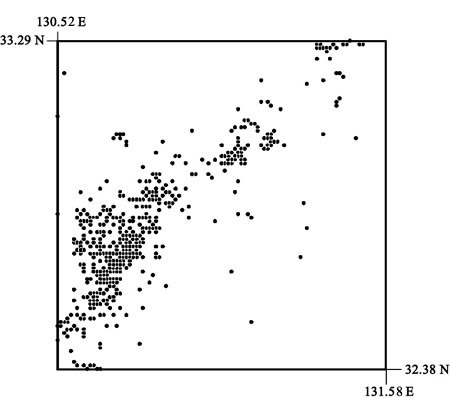
\includegraphics[width=3.83in,height=2.38in]{ris_01_a.png}}
\caption{название рисунка}
\label{fig1}
\end{figure}

Продолжение текста статьи Продолжение текста статьи Продолжение текста статьи Продолжение текста статьи Продолжение текста статьи Продолжение текста статьи Продолжение текста статьи Продолжение текста статьи Продолжение текста статьи Продолжение текста статьи Продолжение текста статьи Продолжение текста статьи Продолжение текста статьи Продолжение текста статьи Продолжение текста статьи Продолжение текста статьи Продолжение текста статьи Продолжение текста статьи Продолжение текста статьи 

Пример размещения двух рисунков
\begin{figure}[ht!]
\begin{minipage}
[b]{0.47\linewidth}
\center{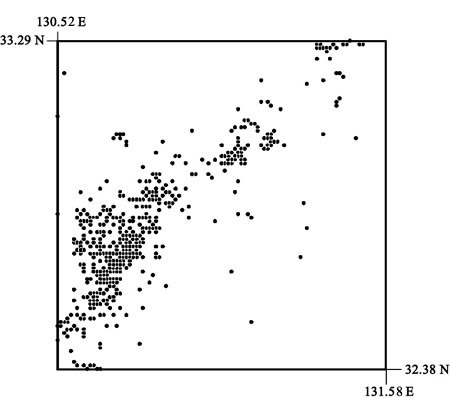
\includegraphics[width=1\linewidth]{ris_01_a.png}} a) \\
\end{minipage}
\hfill
\begin{minipage}[b]{0.5\linewidth}
\center{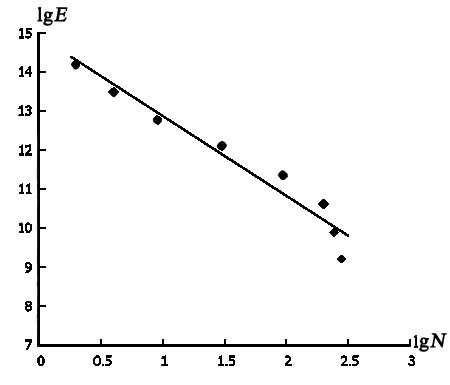
\includegraphics[width=1\linewidth]{ris_01_b.png}} b) \\
\end{minipage}
\caption{а) Пространственное распределение, b) График повторяемости в энергетической}\label{fig:RC2}
\end{figure}

Продолжение текста статьи Продолжение текста статьи Продолжение текста статьи Продолжение текста статьи Продолжение текста статьи Продолжение текста статьи Продолжение текста статьи Продолжение текста статьи Продолжение текста статьи Продолжение текста статьи Продолжение текста статьи Продолжение текста статьи Продолжение текста статьи Продолжение текста статьи Продолжение текста статьи Продолжение текста статьи Продолжение текста статьи Продолжение текста статьи Продолжение текста статьи 

\section*{Заключение}

Продолжение текста статьи Продолжение текста статьи Продолжение текста статьи Продолжение текста статьи Продолжение текста статьи Продолжение текста статьи Продолжение текста статьи Продолжение текста статьи Продолжение текста статьи Продолжение текста статьи Продолжение текста статьи Продолжение текста статьи Продолжение текста статьи Продолжение текста статьи Продолжение текста статьи Продолжение текста статьи Продолжение текста статьи Продолжение текста статьи Продолжение текста статьи 


%%%%%%%%%%%%%%%%%%%%%%%%%%%%%%%%%%%%%%%%%%%%%%%%%%%%%%%%%%%%%%%%%%%%%%%%%%%%%%%%%%%%%%%%%%%

\begin{thebibliography}{99}

\bibitem{Singe}
Синг Дж. 
Общая теория относительности. 
М.: ИЛ, 1963. С. 247--248 

\bibitem{Zakh}
Захаров В.Д. 
Гравитационные волны в теории тяготения Эйнштейна (Современные проблемы физики). 
М.: Наука, 1972. С. 119.

\bibitem{Kennel1} 
Kennel C.F., Petschek H.E. 
Limit on stably trapped particle fluxes. 
{\it J. Geophys. Res.} 1966. V. 71. № 1. 1--14~pp.

\bibitem{Lyons2} 
Lyons L.R., Williams D.J. 
Quantitative aspects of magnetospheric physics. 
N.Y.: Springer, 1984. 312 p.

\bibitem{Nishida1} 
Nishida A. Geomagnetic diagnosis of the magnetosphere. 
N.Y.: Springer-Verlag, 1978. 301 p.

\end{thebibliography}

%%%%%%%%%%%%%%%%%%%%%%%%%%%%%%%%%%%%%%%%%%%%%%%%%%%%%%%%%%%

\begin{otherlanguage}{english}

\begin{thebibliography}{99}

\bibitem{Synge}
Synge J.L. 
{\it Relativity: The General Theory}. 
Amsterdam: North-Holland Publishing Company, 1960.  

%\bibitem{Zakh}
Zakharov V.D. 
{\it Gravitatsionnyye volny v teorii tyagoteniya Eynshteyna (Sovremennyye problemy fiziki)}. 
Moscow: Nauka Publ., 1972. 119 p. (in Russ.)

\bibitem{Kennel} 
Kennel C.F., Petschek H.E. 
Limit on stably trapped particle fluxes. 
{\it J. Geophys. Res.}, 1966, vol. 71, no. 1, pp. 1--14.

\bibitem{Lyons} 
Lyons L.R., Williams D.J. 
{\it Quantitative aspects of magnetospheric physics.} 
N.Y.: Springer, 1984. 312 p.

\bibitem{Nishida} 
Nishida A. 
{\it Geomagnetic diagnosis of the magnetosphere.} 
N.Y.: Springer-Verlag, 1978. 301 p.


\end{thebibliography}

\vspace{10pt}
\begin{otherlanguage}{russian}
\Footer
\end{otherlanguage}

\vspace{10pt}
\FooterSub
\end{otherlanguage}



\end{document}

